%%%%%%%%%%%%%%%%%%%%%%%%%%%%%%%%%%%%%%%%%
% "ModernCV" CV and Cover Letter
% LaTeX Template
% Version 1.11 (19/6/14)
%
% This template has been downloaded from:
% http://www.LaTeXTemplates.com
%
% Original author:
% Xavier Danaux (xdanaux@gmail.com)
%
% License:
% CC BY-NC-SA 3.0 (http://creativecommons.org/licenses/by-nc-sa/3.0/)
%
% Important note:
% This template requires the moderncv.cls and .sty files to be in the same 
% directory as this .tex file. These files provide the resume style and themes 
% used for structuring the document.
%
%%%%%%%%%%%%%%%%%%%%%%%%%%%%%%%%%%%%%%%%%

%----------------------------------------------------------------------------------------
%	PACKAGES AND OTHER DOCUMENT CONFIGURATIONS
%----------------------------------------------------------------------------------------

\documentclass[11pt,a4paper,sans]{moderncv} % Font sizes: 10, 11, or 12; paper sizes: a4paper, letterpaper, a5paper, legalpaper, executivepaper or landscape; font families: sans or roman

\moderncvstyle{classic} % CV theme - options include: 'casual' (default), 'classic', 'oldstyle' and 'banking'
\moderncvcolor{blue} % CV color - options include: 'blue' (default), 'orange', 'green', 'red', 'purple', 'grey' and 'black'

%\usepackage{lipsum} % Used for inserting dummy 'Lorem ipsum' text into the template

\usepackage[scale=0.75]{geometry} % Reduce document margins
%\setlength{\hintscolumnwidth}{3cm} % Uncomment to change the width of the dates column
%\setlength{\makecvtitlenamewidth}{10cm} % For the 'classic' style, uncomment to adjust the width of the space allocated to your name

\usepackage{background}
\backgroundsetup{
scale=1,
angle=0,
opacity=.1,  %% adjust
contents={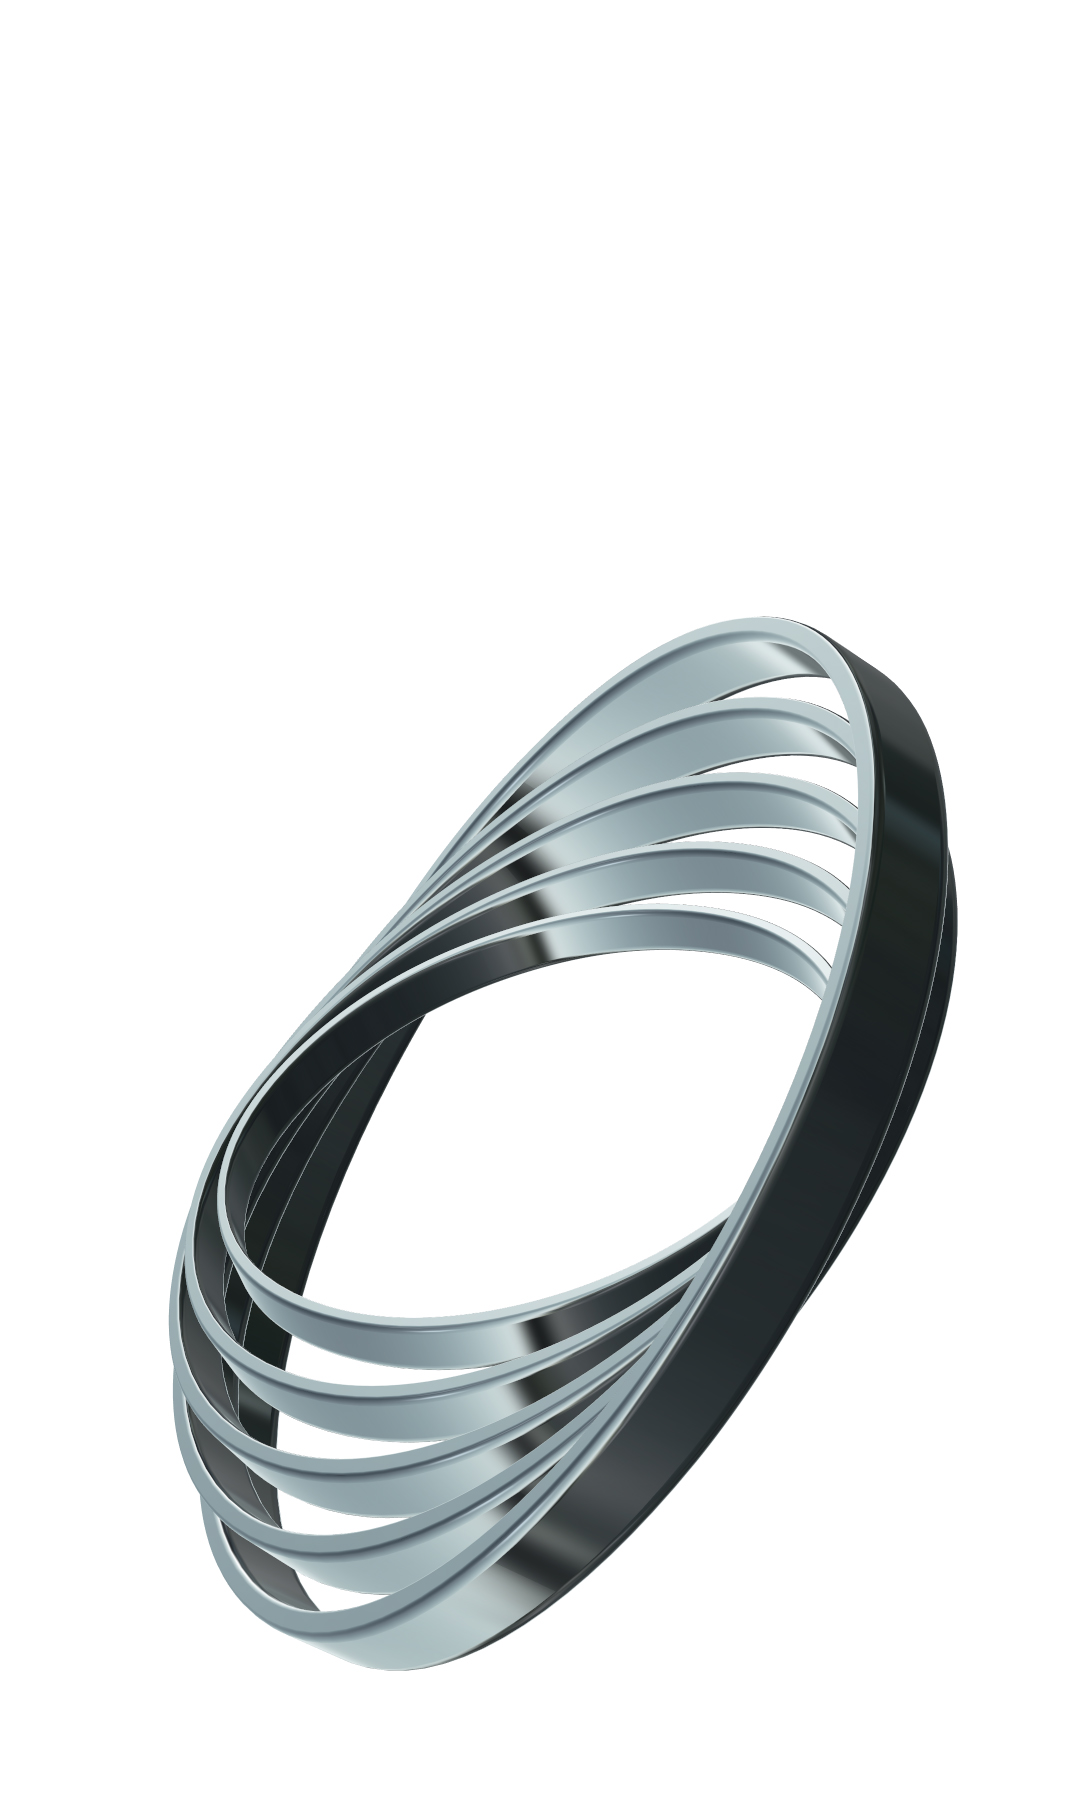
\includegraphics[trim={0 0 0 17cm},width=\paperwidth,height=\paperheight]{pictures/BG5.jpg}}
}
%----------------------------------------------------------------------------------------
%	NAME AND CONTACT INFORMATION SECTION
%----------------------------------------------------------------------------------------

\firstname{Antonius} % Your first name
\familyname{Torode} % Your last name

% All information in this block is optional, comment out any lines you don't need
\title{https://torodean.github.io}
\address{2768 NW 152$^\textrm{nd}$ St. Clive, IA 50325}{}
\mobile{517-512-3580}
%\phone{None}
\email{AWTorode@gmail.com}
%\homepage{https://torodean.github.io}{https://torodean.github.io} % The first argument is the url for the clickable link, the second argument is the url displayed in the template - this allows special characters to be displayed such as the tilde in this example
%\extrainfo{Contact via e-mail is best}
%\photo[70pt][0.4pt]{pictures/picture_me} % The first bracket is the picture height, the second is the thickness of the frame around the picture (0pt for no frame)
%\quote{}

%----------------------------------------------------------------------------------------

\begin{document}

\makecvtitle % Print the CV title


\section{References}

\cventry{2017--2018}{Artemis Spyrou}{Associate Professor of Physics, National Superconducting Cyclotron Laboratory}{Cyclotron, 640 S Shaw Ln, East Lansing, MI 48824}{spyrou@nscl.msu.edu (517)-908-7141}{Supervisor at NSCL.}
\cventry{2016--2018}{Esther V. V. Reed}{Information Technologist Departmental Support, Michigan State University}{Biomed/Physical Science Building: 567 Wilson Road, Room 1209, East Lansing, MI 48824}{reed@pa.msu.edu (517)-884-5469}{Supervisor at Michigan State University.}
\cventry{2017--2018}{Mallory Smith}{Beam Physicist \& Research Scientist, National Superconducting Cyclotron Laboratory}{Cyclotron, 640 S Shaw Ln, East Lansing, MI 48824}{smithma@nscl.msu.edu (517)-908-7186}{Post-Doctorial researcher at NSCL.}
\cventry{2013--2015}{Michael Robinson}{Faculty, Oakland Community College}{739 S Washington Ave, Royal Oak, MI 48067}{mdrobins@oaklandcc.edu (248)-232-4438}{Employer at Oakland Community College.}
\cventry{2011--2013}{Mitch Kanaan}{President/Owner, CLRS, inc.}{29433 Southfield Road, Suite 106 Southfield, Michigan 48076}{mkanaan@clrsinc.com (248)-760-5316}{Employer at CLRS, Inc.}

%----------------------------------------------------------------------------------------
%	COVER LETTER
%----------------------------------------------------------------------------------------

% To remove the cover letter, comment out this entire block

%\clearpage

%\recipient{HR Department}{Corporation\\123 Pleasant Lane\\12345 City, State} % Letter recipient
%\date{\today} % Letter date
%\opening{Dear Sir or Madam,} % Opening greeting
%\closing{Sincerely yours,} % Closing phrase
%\enclosure[Attached]{curriculum vit\ae{}} % List of enclosed documents

%\makelettertitle % Print letter title

%\lipsum[1-3] % Dummy text

%\makeletterclosing % Print letter signature

%----------------------------------------------------------------------------------------

\end{document}